% background of problem solved
% existing solutions
% reading and research
% !!!Project requirement
\section{Background}
\subsection{The problem to be solved}

\subsection{Existing solution}

\subsection{Brief Introduction to Population Protocols \label{background} \cite{AspnesR2007, MCS11}}
\par\noindent
Population protocols are theoretical models for distributed computation.
The model contains a collection of indistinguishable agents.
They (i.e. the agents) carry out computation tasks through directly pair-wised interactions.
The interaction pattern of agents is unpredictable from perspective of agents themselves
and is controlled through an adversary scheduler with fairness constraints.
\paragraph{Formal Definition}
A protocol can be formally defined as:
\begin{itemize}
  \item $Q$, a finite set of passible states for an agent,
  \item $\Sigma$, a finite set of input alphabet,
  \item $Y$, a finite set of output range,
  \item $\iota = \Sigma \to Q $, is an input map from $\sum$ to $Q$, hence $\iota(\sigma)$ represents the initial state whose input is $\sigma \in \Sigma$
  \item $\omega = Q \to Y $, is an output map from $Q$ to $Y$, and
  \item $\delta \subseteq Q^{4}$, a transition relation describes how pairs of agents can interact.
\end{itemize}


\par\noindent
A \textit{configuration} for a population is a vector of all the agents' states.
Because agents with a same state are indistinguishable with each other, each configuration
could also an unordered multiset of states. It can be represented as $C$.


\par \label{IntroToPPFairScheduler} \noindent
At any point of the discrete time, the interaction is unpredictable from the perspective of the agents
in the population and the population itself. The interactions at any time are decided
by a adversary scheduler necessarily enforced with \textit{fairness} condition.
The fairness condition means that the scheduler cannot avoid a possible step forever.
Formally, it means if a infinitely often configuration $C$ and $C \to C^{'}$,
the $C^{'}$ must also appear infinitely of in the execution.


\begin{figure}[H]
\begin{center}
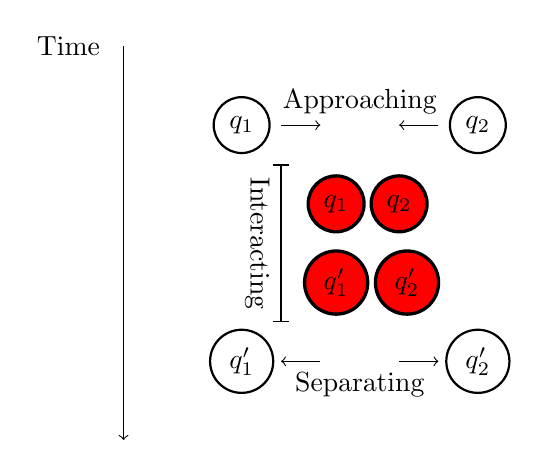
\begin{tikzpicture}
    [L0Node/.style={circle,   draw=black, thick, minimum size=7mm},
    L1Node/.style={circle,   draw=black, fill=red, very thick, minimum size=7mm}]
     \node[L0Node] (n0) at (0, 2){$q_1$};
     \node[L0Node] (n1) at (3, 2){$q_2$};
     \node[L1Node] (n2) at (1.2, 1){$q_1$};
     \node[L1Node] (n3) at (2.0, 1){$q_2$};
     \node[L1Node] (n4) at (1.2, 0){$q'_{1}$};
     \node[L1Node] (n5) at (2.1, 0){$q'_{2}$};
     \node[L0Node] (n6) at (0, -1){$q'_{1}$};
     \node[L0Node] (n7) at (3, -1){$q'_{2}$};
     \draw[->] (0.5,2) -- (1.0, 2);
     \draw[<-] (2,2) --  (2.5,2);
     \draw[<-] (0.5,-1) -- (1.0, -1);
     \draw[->] (2,-1) --  (2.5,-1);
     \draw[->] (-1.5,3) -- (-1.5, -2);
     \draw[|-|] (0.5,-0.5) -- (0.5,1.5);
     \node (TimeLabel) at (-2.2, 3){Time};
     \node (ApproachingLabel) at (1.5, 2.3){Approaching};
     \node (SeparatingLabel) at (1.5, -1.3){Separating};
     \node[rotate=-90]  (InteractingLabel) at (0.2, 0.5){Interacting};
\end{tikzpicture}
\end{center}
\caption{A typical (simple) interaction in population protocol}
\end{figure}



\par\noindent
The current implementation of this work assumes a more strict scheduler called random scheduler,
which resulting uniform random interactions (i.e. at each step, it presents
equally possibility for every pair of agents to interact.) Essentially, a random scheduler is a "fair" scheduler, but a "fair" scheduler is not necessarily a random scheduler.
The assumption actually increases the power of the model because it allows a leader agent detects the absence
of agents in a particular state after a long enough waiting. Note this is only for
simplifying the current implementation and possibly extends to other fair schedulers that is not a
random scheduler in the future.

\subsection{From Population Protocols to Network Constructor \cite{MS16a}}

\par\noindent
A variance of population protocol is called "network constructor" \cite{MS16a}.
It involves the extra elements do not existing in general population protocol called "edge", which is
the connection in between any two agents (or "processes"). In general, the connection
is similar to the agents, on the characteristic that they all only have a finite number of states. For instance, if
a connection have $k + 1$ states,  state 0 may represent the connection does not exist and for state $i \in \{1,2,3, ..., k\}$
shows the strength for a particular connection.


\par\noindent
In the following paragraph and the currently implemented simulator, we solely consider the simplest
case containing only $on$ and $off$ two states for edges. A connection is said to be in
$on$ or $active$ state, if at any discrete time, the connection exists in between two
particular nodes; otherwise if the connection is stated as in $off$ or $inactive$ state.
At initial, all edge are in $off$ state, which means that there is no connection in a given
population at discrete time 0. The state for an edge may or may not change through an interaction
in between the two nodes it connected or disconnected to.


\par\noindent
The network constructor also follows an adversary scheduler with "fairness" constraint. This is
exactly same as the paragraphs mentioned in the previous section \ref{IntroToPPFairScheduler}.

\paragraph{Formal Definition}
Formally, a network constructor can be defined as:
\begin{itemize}
  \item $Q$, a finite set of passible states for an agent,
  \item $Q_{out}$, a finite set of output range,
  \item $q_{0} \in Q $, is initial state of node,
  \item $\delta: Q \times Q \times \{0,1\} \to Q \times Q \times \{0,1\}$, a transition function, where the $\{0,1\}$ is the states for edges with initial value 0.
\end{itemize}


\par\noindent
The main target of this model concentrates on network construction rather than
specific function computation, which is the task for general population protocol. Notice that a transition can be either \textit{effective}
or \textit{ineffective}. Define $\delta(a, b, c) = (a^{'}, b^{'},c^{'})$ as a transition function (Here, $a, b$ are "node-state" whereas $c$ is state for edge.)
as it is in the formal definition, $\delta_{1}(a,b,c) = a^{'}$, $\delta_{2}(a,b,c) = b^{'}$ (representing two nodes states' change)
and $\delta_{3}(a,b,c) = c^{'}$ (representing edge state change), the transition $(a,b,c) \to (a^{'}, b^{'},c^{'})$ is called
effective if at least one $x \in \{a,b,c\} \not= x^{'} $; otherwise it is called ineffective.


\par\noindent
Name the set of nodes (or "distributed processes" under this context) $V_{I}$ and the set of pairs of nodes as $E_{I}$.
A configuration $C$ is a mapping $ V_{I} \cup E_{I} \to Q \cup \{0,1\} $ determines the states of nodes and edges in the population at any discrete time.
The output of configuration $C$ is defined as the graph $G(C) = (V, E) $ where $V = \{u \in V_{I}: C(u) \in Q_{out}\}$
and  $E = \{uv: u, v \in V, u \not= v,$ and $C(uv) = 1\}$.

\subsection{Grid Terminating Network Constructor \cite{Mi17} \label{IntroToGrid}}

\par\noindent
Another paper \cite{Mi17} presents a different automata but very similar to network constructor. Each node in this
model has a fixed number of ports with it. In the 2-dimensional case, it will have 4 distinguished ports
$p_{y}$, $p_{x}$, $p_{-y}$ and $p_{-x}$, may simply donated as $u$, $r$, $d$ and $l$, respectively.
The port, which neighbour with each other, are also perpendicular to each other, forming local axes. Hence,
$ u \perp r $, $ r \perp d $, $ d \perp l $, and  $ l \perp u $. The coordinates are only for local purposes and
do not necessarily represent the actual orientation of a node. A connection (or edge) can only be built through
pairs of ports, which is different from the previous model (network constructor).


\par\noindent
\begin{figure}[H]
\begin{center}
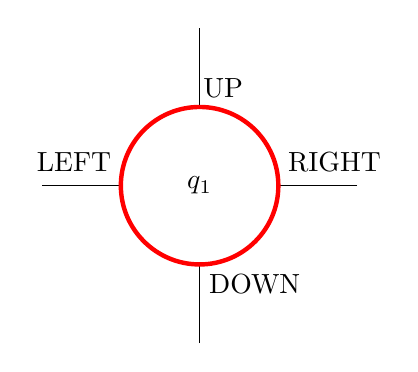
\begin{tikzpicture}
    \draw (2,0) -- (2,1);
    \draw (2,4) -- (2,3);
    \draw (0,2) -- (1,2);
    \draw (4,2) -- (3,2);
    \draw [red, ultra thick] (2,2) circle [radius=1];
    \node [below] at (2.7,1) {DOWN};
    \node [above] at (2.3,3) {UP};
    \node [left] at (1,2.3) {LEFT};
    \node [right] at (3,2.3) {RIGHT};
    \node [label] at (2,2) {$q_1$};
\end{tikzpicture}
\end{center}
\caption{Structure of a node in Grid Terminating Network Constructor model}
\end{figure}


\par\noindent
\paragraph{Formal Definition}
Formally, a terminating grid network constructor in 2-D can be defined as:
\begin{itemize}
  \item $Q$, a finite set of passible states for an agent,
  \item $Q_{out}$, a finite set of output range,
  \item $q_{0} \in Q $, is initial state of node
  \item $\delta: (Q \times P ) \times (Q \times P) \times \{0,1\} \to Q \times Q \times \{0,1\}$, a transition function, where the $\{0,1\}$ is the states for edges with initial value 0.
  \item When required, there will be also a special initial leader-state $L_{0} \in Q $ defined.
\end{itemize}

\par\noindent
A transition can be either \textit{effective}
or \textit{ineffective}. Define $\delta((a, p_{1}), (b, p_{2}), c) = (a^{'}, b^{'},c^{'})$ as a transition function
as it is in the formal definition, it is called effective if at least one $x \in \{a,b,c\} \not= x^{'} $; otherwise it is called ineffective.


\par\noindent
Every configuration $C$ forms a set of shapes $G[A(C)]$, where a shape means that the network induced
by active edges of $C$. Given the geometrical restrictions (i.e. the connection are
made at unit distance and are perpendicular whenever they correspond to consecutive ports of a node),
not all possible $A(C)$ are valid. $A(C)$ is valid if any connected component defined by it is a
subnetwork of 2D grid network with unit distances. A valid $A(C)$ at time $t -1$ also restricts the
possible valid $A(C)$ at time $t + k$, where $k \in Integer$ and $k \geq 0 $.


\par\noindent
The paper \cite{Mi17} also defines a set of
shapes $G_{out}(C) = \{V_{s}, E_{s}\}$ as output of a configuration where $V_{s} = \{u \in V : C_{v}(u) \in Q_{out} \}$
and $E_{s} = A(C) \cap \{ (v_{1}, p_{1}) : v_{1} \not= v_{2} \in V_{s}; p_{1}, p_{2} \in P \}$.
Less formally, the output shapes of a configuration contains all nodes in output states and the active edges in between them.
This model focuses on terminating protocols so it assumes $Q_{out} \subseteq Q_{halt} \subseteq Q $.
All rules containing $q_{halt} \in Q_{halt} $ is ineffective.

\subsection{Vector transformation: handle coordinate rotations in 2-dimension}


\par\noindent
As mentioned in the previous section \ref{IntroToGrid}, Grid Terminating Network Constructor enforces perpendicular ports
and geometrical restrictions. This means that handling rotation in some cases becomes necessary.
This section will cover some basic but related vector mathematics. The detailed algorithms will be discussed later on, in the "Realisation" section (\ref{Realisation}).

\subsubsection{2D centred coordinate rotation, with origin point as the centre}

\par\noindent

\begin{figure}[H]
\begin{center}
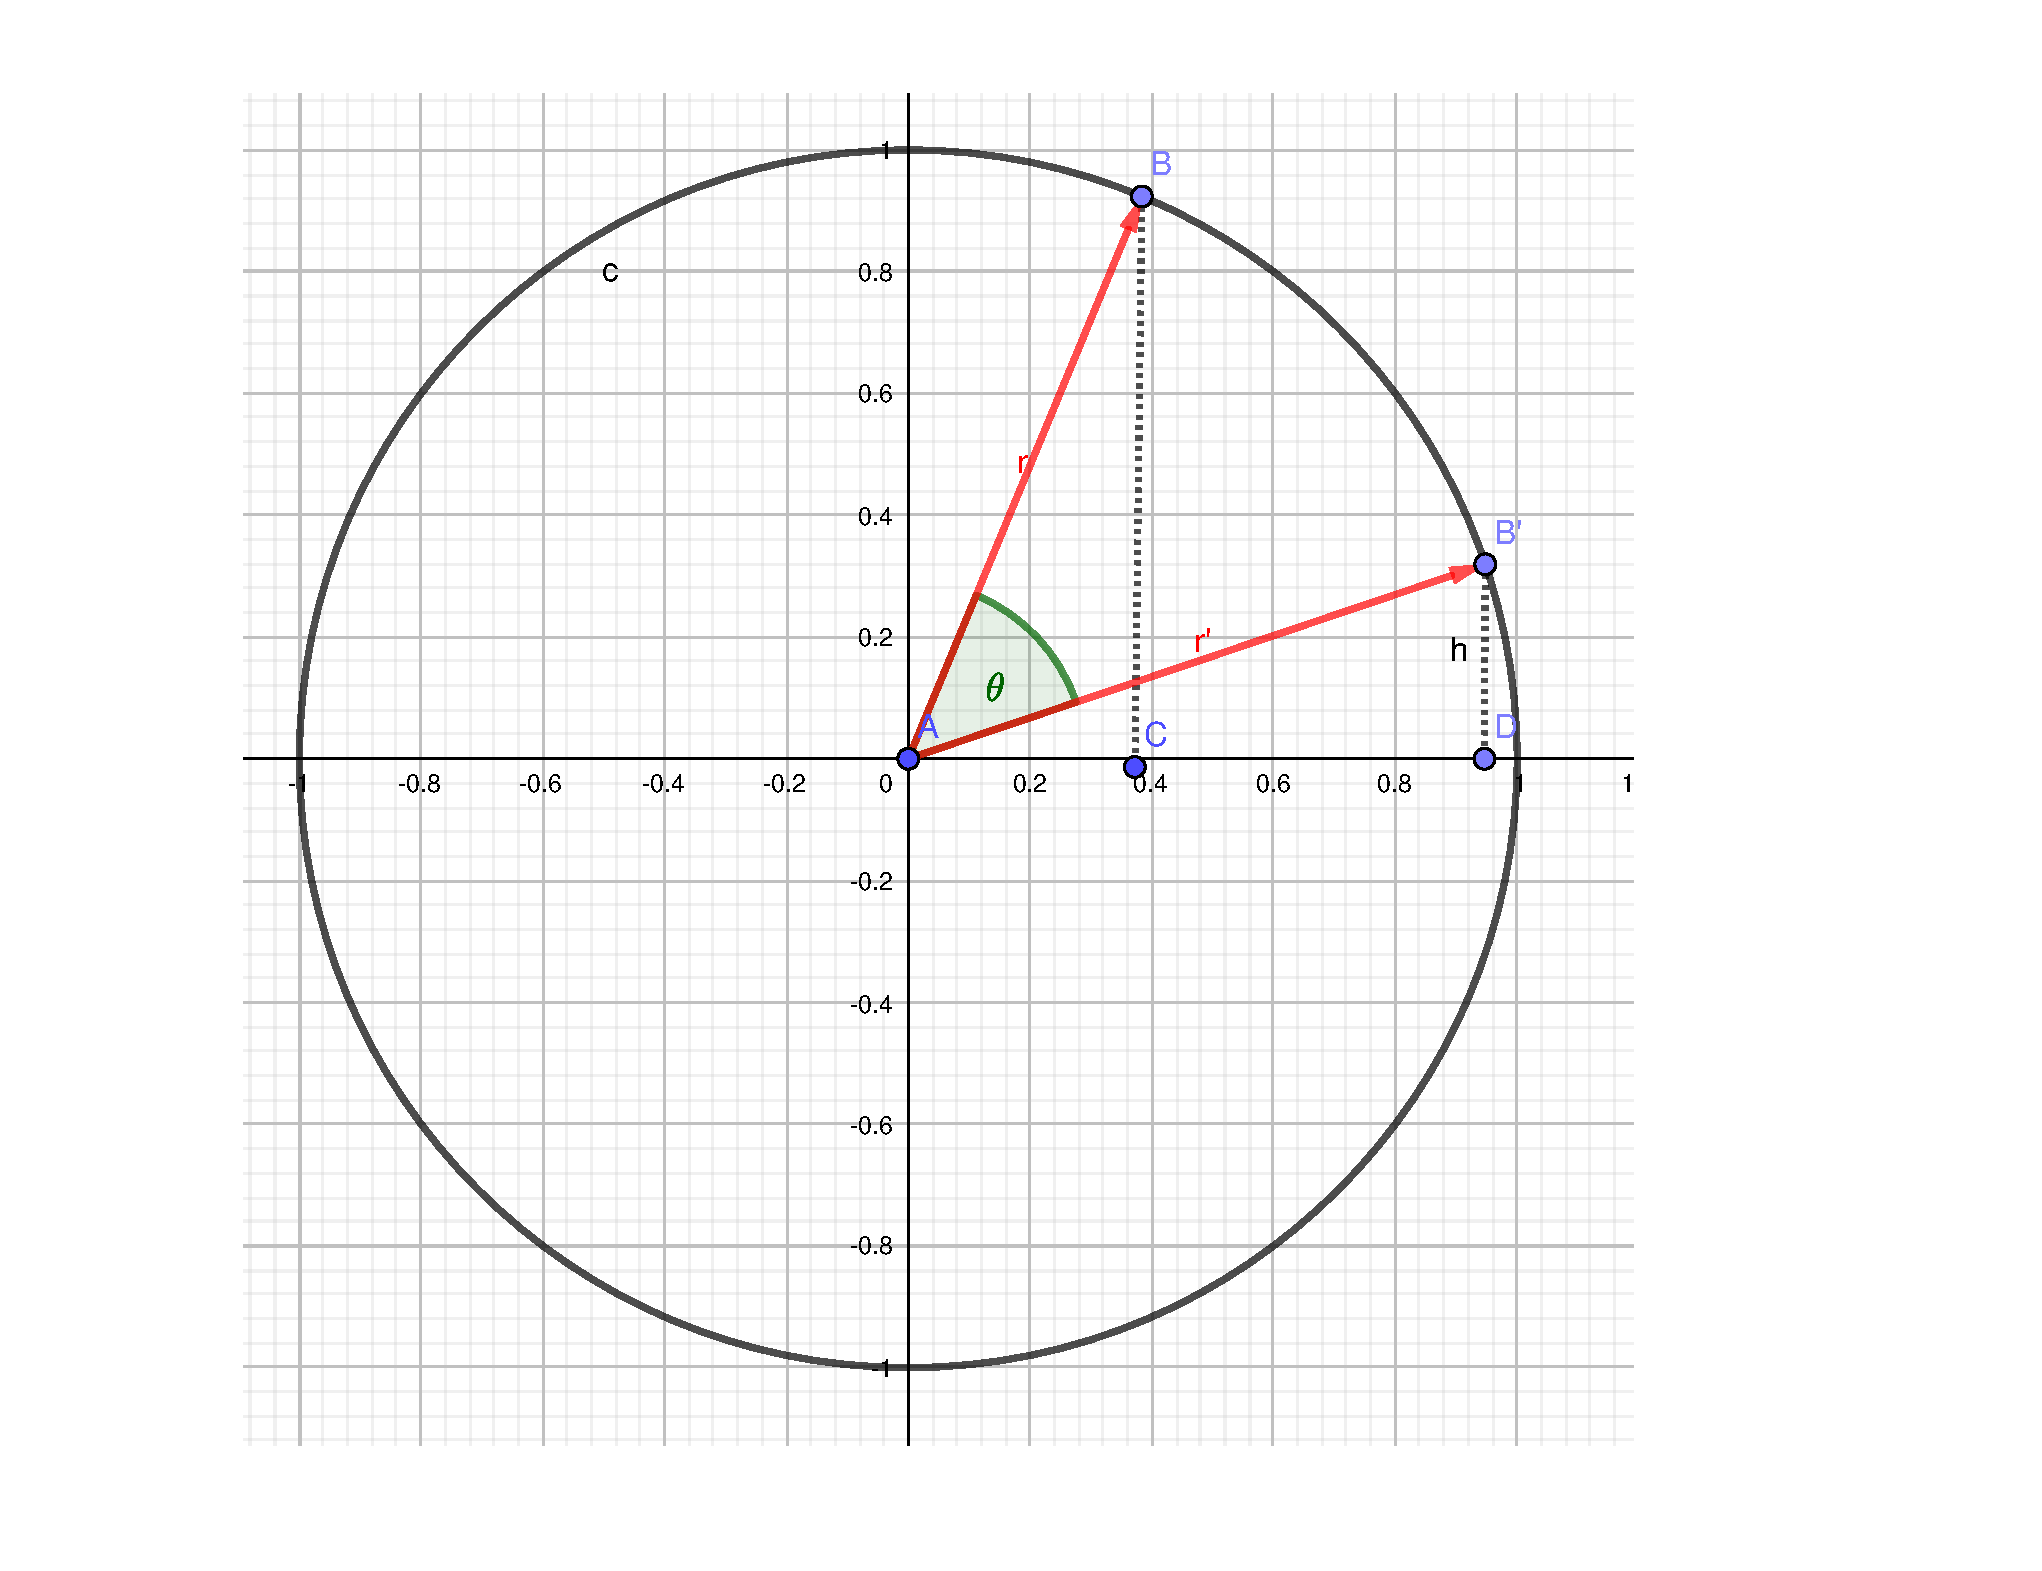
\includegraphics[width=0.6\textwidth]{context/diagram/2d_vector.pdf}
\caption{Vector $\vec{r}$ and $\vec{r_{'}}$ in unit circle}

\label{vectorG}
\end{center}
\end{figure}

\par\noindent
The figure \ref{vectorG} has two same-length vectors,  $\vec{r}$ (or $\vec{AB}$) and $\vec{r_{'}}$ (or $\vec{AB_{'}}$) in its Cartesian coordinate and their destination point located at the same unit circle.
The point $A$ is the origin point with coordinate $(0, 0)$. Suppose it has already known for the coordinate of $B$ is
$(x,y)$, and the $\theta$ angle. The question is that what the coordinate of $B^{'} $ (representing in $(x^{'},y^{'})$) is, after the first vector $\vec{r}$ rotates the given angle $\theta$ and becomes $\vec{r_{'}}$.
Note that, the "positive" rotation direction in current context and the implementation of the simulator is defined as "clock-wised".

\par\noindent
To solve this, the following equation can be concluded:

\begin{equation} \label{Equ_ori}
  \begin{bmatrix}
   x^{'} \\ y^{'}
   \end{bmatrix} =   \begin{bmatrix}
      \cos\theta & \sin\theta \\
      -\sin\theta & \cos\theta
    \end{bmatrix} \begin{bmatrix}
      x \\ y
     \end{bmatrix}
\end{equation}


\par\noindent
A brief proof can be found in appendix partition below and it also can be found in \cite{Mitnote09} with a more precise and general proof.


\subsubsection{2D centred coordinate rotation, with any points as the centre}
Given the equation (\ref{Equ_ori}), it can be easily
deduced that the rotation equation for any centred points $c$ with coordinate $(c_{x}, c_{y})$ can be achieved through
panning $c$ to origin point with coordinate $(0, 0)$, carry out the rotation and panning back to its original coordinate $(c_{x}, c_{y})$.
Suppose the target point that is required to be rotated is called $p$ (with coordinate $(x, y)$), it then has :
\begin{equation} \label{Equ_anycen}
  \begin{bmatrix}
   x^{'} \\ y^{'}
   \end{bmatrix} =   \begin{bmatrix}
      \cos\theta & \sin\theta \\
      -\sin\theta & \cos\theta
    \end{bmatrix} \left(\begin{bmatrix}
      x \\ y
     \end{bmatrix} - \begin{bmatrix}
       c_{x} \\ c_{y}
     \end{bmatrix}\right) + \begin{bmatrix}
        c_{x} \\ c_{y}
       \end{bmatrix}
\end{equation}

\subsubsection{Affine transformation form}
After a series of transformation, the equation \ref{Equ_anycen} becomes the following form:

\begin{equation} \label{Equ_aff}W
  \begin{bmatrix}
   x^{'} \\ y^{'}
   \end{bmatrix}  = \begin{bmatrix} \cos\theta & \sin\theta \\ -\sin\theta & \cos\theta \end{bmatrix} \begin{bmatrix} x \\ y \end{bmatrix}
+ \begin{bmatrix} c_{x}(1 - \cos\theta) - c_{y}\sin\theta \\ c_{y}(1 - \cos\theta) + c_{x}\sin\theta \end{bmatrix}
\end{equation}

\par\noindent
Let $ \textbf{M} = \begin{bmatrix} \cos\theta & \sin\theta \\ -\sin\theta & \cos\theta \end{bmatrix} $
and $ \textbf{B} = \begin{bmatrix} c_{x}(1 - \cos\theta) - c_{y}\sin\theta \\ c_{y}(1 - \cos\theta) + c_{x}\sin\theta \end{bmatrix}$, then $ \begin{bmatrix} x^{'} \\ y^{'} \end{bmatrix}  = \textbf{M} \begin{bmatrix} x \\ y \end{bmatrix} + \textbf{B}$,
where it forms an \textit{affine transformation} \cite{WolframAT}. \textbf{M} and \textbf{B} can be calculated directly after knowing the rotation centre $(c_{x}, c_{y})$ and the
rotation agle $\theta$, and therefore the calculated \textbf{M} and  \textbf{B} can be applied for multiple target coordinates (those coordinates required to be rotated). This simplifies the calculation for a large batch of centred rotation with multiple target coordinates.




% \section {Data required} see website
% \section {Realisation \label{Realisation}} each stage & component; discuss problem encountered problem and solutions; testing (for each component); snapshot
% \section {Experiment  (optional)} propose; design of exp. ; exp. settings; discussion of results; chart and explain for chart
% \section {Evaluation} successful or not; how evaluate; who evaluate the project; strength and weakness of the project
% \section {Learning Points} [at least one page], story
% \section {Professional issues}  [at least one page] British Computer Society related to the project: Code of practice; Code of conduct
% \section Bio
% \section{Appendix} details of test data; (optional)more screen shot of sample; use guide; full design diagram
% zip of project
